%%%%%%%%%%%%%%%%%%%%%%%%%%%%%%%%%%%%%%%%%
% Wenneker Assignment
% LaTeX Template
% Version 2.0 (12/1/2019)
%
% This template originates from:
% http://www.LaTeXTemplates.com
%
% Authors:
% Vel (vel@LaTeXTemplates.com)
% Frits Wenneker
%
% License:
% CC BY-NC-SA 3.0 (http://creativecommons.org/licenses/by-nc-sa/3.0/)
% 
%%%%%%%%%%%%%%%%%%%%%%%%%%%%%%%%%%%%%%%%%

%----------------------------------------------------------------------------------------
%	PACKAGES AND OTHER DOCUMENT CONFIGURATIONS
%----------------------------------------------------------------------------------------

\documentclass[12pt]{scrartcl} % Font size
\usepackage{hyperref} 
\usepackage{graphicx}
%----------------------------------------------------------------------------------------
%	TITLE SECTION
%----------------------------------------------------------------------------------------

\title{	
	\normalfont\normalsize
	\textsc{Brown University}\\ % Your university, school and/or department name(s)
	\vspace{25pt} % Whitespace
	\rule{\linewidth}{0.5pt}\\ % Thin top horizontal rule
	\vspace{20pt} % Whitespace
	{\huge Finding Motifs Using Gibbs Sampling}\\ % The assignment title
	\vspace{12pt} % Whitespace
	\rule{\linewidth}{2pt}\\ % Thick bottom horizontal rule
	\vspace{12pt} % Whitespace
}

\author{\LARGE Anirudh Narsipur} % Your name

\date{\normalsize\today} % Today's date (\today) or a custom date

\begin{document}

\maketitle % Print the title

%----------------------------------------------------------------------------------------
%	FIGURE EXAMPLE
%----------------------------------------------------------------------------------------

\section{Introduction}

Finding motifs for transcription factors is important in the study of
transcription factors. However, finding correct motifs efficiently is not trivial.
\newline \newline 
Here I implement Gibbs Sampling, a heavily studied algorithm for finding motifs. I apply this algorithm
to find motifs for transcription factors in Mycobacterium tuberculosis (MTB) and discuss my results.
\section{Background}
Within each cell, DNA gets transcripted into RNA which is then translated into
protein. The amount of expression of a protein and it's timing is strictly controlled.
This ensures that proteins are expressed at the correct stage in the cell life cycle or not expressed
at all. Transcription factors (TF) are an important part of this regulatory framework.

Transcription factors are proteins that bind slightly upstream of the genes they regulate.
They either promote (activators) or block (repressors) gene transcription by RNA polymerase.
Transcription factors are usually highly specific and bind to specific sequences known as DNA binding domain (DBD).DBDs contain
a sequence motif that is a conserved DNA sequence. Transcription factors have one or more motifs associated with them and they only bind
at locations where the motif is present. 

Thus it important to identify motifs associated with each transcription factor in order
to study and classify them. Through experimental techniques, such as ChIP-Seq the sequences around the binding sites of transcription factor
can be identified. The computational task is to then identify the motif given the sequence data.

In this project I use Gibbs Sampling to identify motifs and then apply it to Chip-Seq data to identify the motifs in Mycobacterium tuberculosis.
Gibbs Sampling is a probabilistic algorithm that iteratively works towards optimal motifs. From the algorithm we can extract motifs as 
position weight matrices (PWM).

\begin{center}
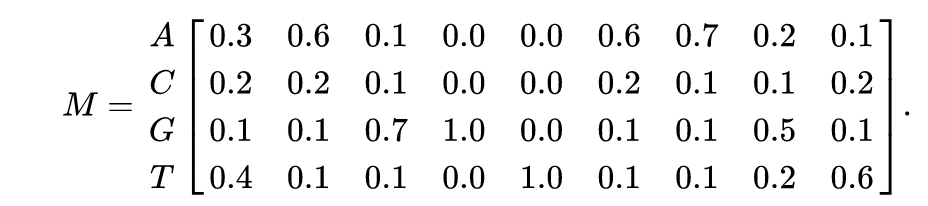
\includegraphics[width=0.5\textwidth]{PWM_Example.png}
\newline Fig 1. An example of a Position Weight Matrix (PWM) \newline for a DNA sequence of length 9. 
\end{center}

Position weight matrices as given above represent a motif by the probability of a each nucleotide being present at a given position. 

\section{Methods}
To rigorously frame our problem of find motifs: 

\emph{Given $n$ DNA sequences $s$ of length $L$, and a target 
motif length $k$, find a $k-mer$ in each string $s_i$ such that distance between $s_i$ and $s_j$ is minimized. $\forall i , j \in \{1,n\}$}

We then use Gibbs Sampling to solve it. Gibbs Sampling proceeds iteratively in the following manner:
\begin{center}
    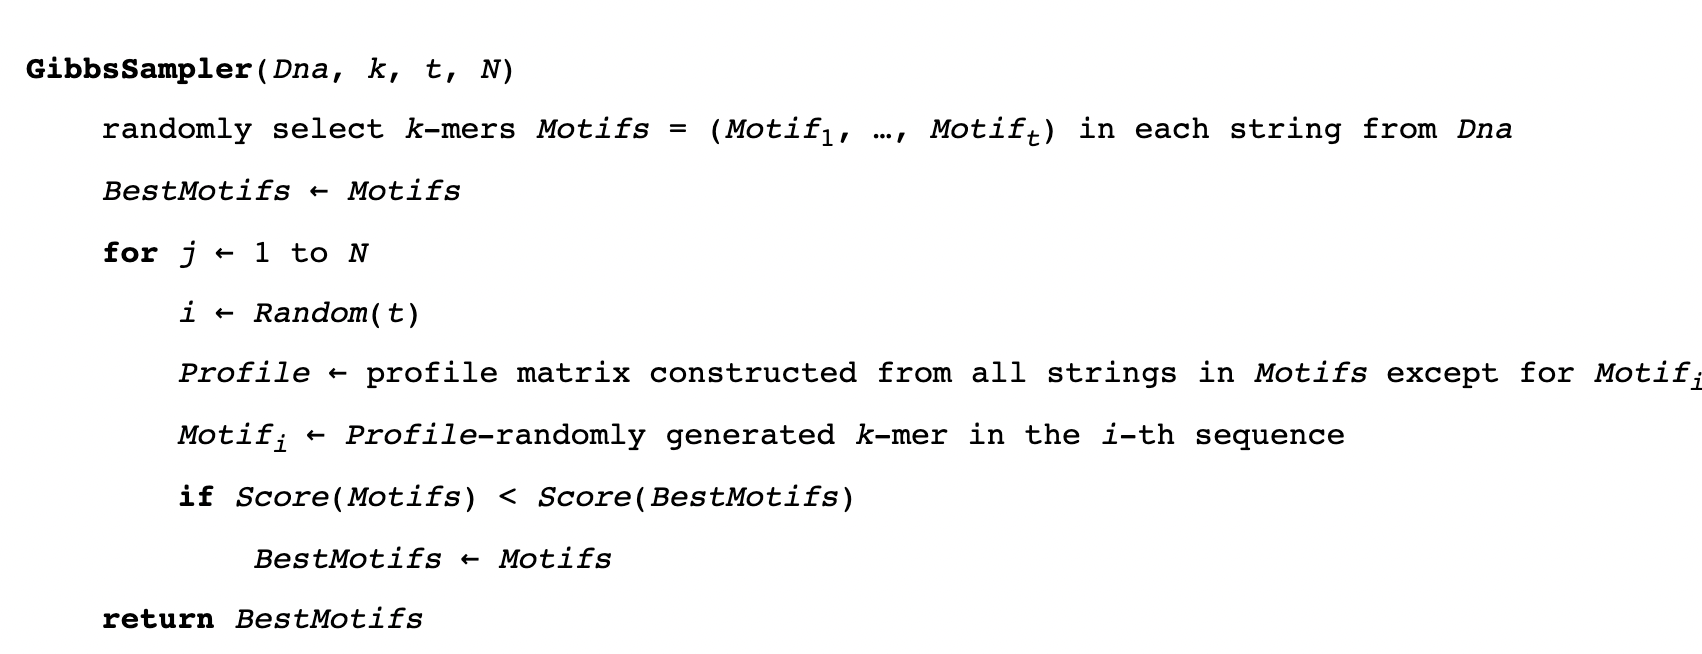
\includegraphics[width=0.95\textwidth]{Pseudocode.png}
    \newline Fig 2. Pseudocode for Gibbs Sampling.
\end{center}

\begin{itemize}
    \item In each string $s_i$, pick a random $k-mer$ $x_i$.
    \item Randomly select a string $s_j$ from the set of strings $s$.
    \item Construct a profile matrix $P$ from the strings $s - \{s_j\}$.
    \begin{center}
        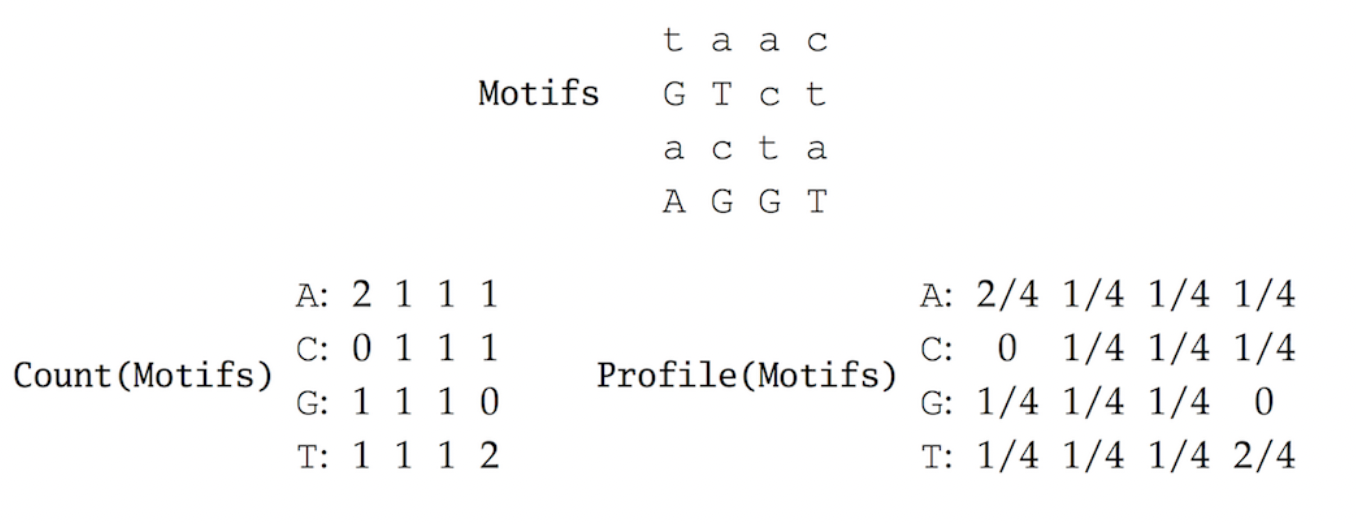
\includegraphics[width=0.95\textwidth]{Profile_m.png}
        \newline Fig 3. Construction of the profile matrix.
    \end{center}
    The profile matrix $P$ is constructed by taking the count of each nucleotide in each position of the strings and then dividing by the total
    number of sequences considered ($n-1$). However, observe that some values are zero. This leads to problems in scoring k-mer as given below. 
    Having a value of zero in the first column of the profile matrix for C indicates that probability of motif starting with C is mathematically zero.This is biologically not true
    as even if a $C$ does not occur at the first nucleotide in the best motif we find later that does not mean the chance of it occurring is zero. 
    \newline 
    To correct for this we add a "pseudocount" to the profile matrix. While more sophisticated methods exist, here we use a simplistic method based on Laplace's rule of succession, that is for
    each value in the profile matrix $m$ we do $\frac{m+1}{(n-1) + 4}$.

    \item Score all $k-mers$ in $s_j$ against the profile matrix $P$.
    $k-mer$ are score by simply taking the product of the probability of each nucleotide at each position in the k-mer as given in the profile matrix.
    To put it more formally, $$Score(x) = Pr(x|P) = \prod_{i=1}^{L}e_i(x_i)$$ where $e_i(x_i)$ is the probability of observing the $i'th$ in $x$ given $M$.
    \item Normalize the resulting probabilities to get a probability distribution $D$.
    For a given sequence we have $w = L - k + 1$ possible k-mers. If our scores are $c_1 ... c_w$ ,then $D = \{  \frac{c_i}{\sum_{j=1}^{w} c_j} , \forall i \in [1,w] \}$. To put it simply, we divide
    each probability by the sum of all probabilities.
    \item Sample a new motif $x_j$ from the probability distribution $D$.
    \item Repeat the above process until convergence or for a set number of iterations.
\end{itemize}
 
\subsection{Background Model}
The above model fails to consider several biological facts:
\begin{itemize}
    \item Nucleotides are not independent.
    The probability of observing a nucleotide $x_i$ in a given position $i$ is not independent of the sequence preceding it.
    \item Nucleotides are usually not equally distributed, and many organisms tend to be either GC dominant or AT dominant. These percentages can significantly
    vary in different parts of the genome.
    \item Repeated sequences can be a confounding factor. For example, $GGG$ could be a common repetition across sequences but not part of a motif.
\end{itemize}

A powerful way to overcome these limitations is to use a background model $B$.A background model 
$B_i$ has order $i$ indicating that the probability of observing a nucleotide depends on $i$ previous
nucleotides.

\section{Results}
\section{Acknowledgements}
This project is a study of well established methods and as such would not possible without existing literature.A special debt is owed
to Bioinformatics Algorithms by Compeau and Pevzner from where all figures are taken from. All data used in this project is drawn from 
Minch et al. (2015). 
\section{References}
\begin{itemize}
    \item Phillip Compeau, Pavel Pevzner (2011). \textsc{
        Bioinformatics Algorithms}.\href{https://www.bioinformaticsalgorithms.org}{Link}
    \item Minch, K., Rustad, T., Peterson, E. et al. The DNA-binding network of Mycobacterium tuberculosi s. Nat Commun 6, 5829 (2015). https://doi.org/10.1038/ncomms6829
    \item Thijs G, Lescot M, Marchal K, Rombauts S, De Moor B, Rouzé P, Moreau Y. A higher-order background model improves the detection of promoter regulatory elements by Gibbs sampling. Bioinformatics. 2001 Dec;17(12):1113-22. doi: 10.1093/bioinformatics/17.12.1113. PMID: 11751219.
    \item A Gibbs Sampling Method to Detect Overrepresented Motifs in the Upstream Regions of Coexpressed Genes
    Gert Thijs, Kathleen Marchal, Magali Lescot, Stephane Rombauts, Bart De Moor, Pierre Rouzé, and Yves Moreau
    Journal of Computational Biology 2002 9:2, 447-464
    \item Seshasayee AS, Sivaraman K, Luscombe NM. An overview of prokaryotic transcription factors : a summary of function and occurrence in bacterial genomes. Subcell Biochem. 2011;52:7-23. doi: 10.1007/978-90-481-9069-0\_2. 
    
    PMID: 21557077.
    
    \item Lawrence CE, Altschul SF, Boguski MS, Liu JS, Neuwald AF, Wootton JC. Detecting subtle sequence signals: a Gibbs sampling strategy for multiple alignment. Science. 1993 Oct 8;262(5131):208-14. doi: 10.1126/science.8211139. PMID: 8211139.
    
    \item George Casella ,  Edward I. George (1992) Explaining the Gibbs Sampler, The
    American Statistician, 46:3, 167-174, DOI: 10.1080/00031305.1992.10475878
\end{itemize}
\end{document}
